
\documentclass[12pt, a4paper, notitlepage]{report}

\usepackage{geometry}
\geometry{a4paper, portrait, margin=1in}

%Sort out generous chapter spacing
\usepackage{titlesec}
\titleformat{\chapter}[display]
{\normalfont\huge\bfseries}{\chaptertitlename\ \thechapter}{10pt}{\Huge} % Was:{\normalfont\huge\bfseries}{\chaptertitlename\ \thechapter}{20pt}{\Huge}
% Make {\scshape\Huge} for ALL chapters to have small caps headings
% Note this does not apply to ToC, but DOES apply to list of tables etc.
\titleformat{\section}
{\normalfont\Large\bfseries}{\thesection}{1em}{}
\titleformat{\subsection}
{\normalfont\large\bfseries}{\thesubsection}{1em}{}
\titleformat{\subsubsection}
{\normalfont\normalsize\bfseries}{\thesubsubsection}{1em}{}
\titleformat{\paragraph}[runin]
{\normalfont\normalsize\bfseries}{\theparagraph}{1em}{}
\titleformat{\subparagraph}[runin]
{\normalfont\normalsize\bfseries}{\thesubparagraph}{1em}{}

\titlespacing*{\chapter} {0pt}{-20pt}{10pt} %Was: {0pt}{50pt}{40pt}
\titlespacing*{\section} {0pt}{3.5ex plus 1ex minus .2ex}{2.3ex plus .2ex}
\titlespacing*{\subsection} {0pt}{3.25ex plus 1ex minus .2ex}{1.5ex plus .2ex}
\titlespacing*{\subsubsection}{0pt}{3.25ex plus 1ex minus .2ex}{1.5ex plus .2ex}
\titlespacing*{\paragraph} {0pt}{3.25ex plus 1ex minus .2ex}{1em}
\titlespacing*{\subparagraph} {\parindent}{3.25ex plus 1ex minus .2ex}{1em}
%\titlespacing{command}{left spacing}{before spacing}{after spacing}[right]
% spacing: how to read {12pt plus 4pt minus 2pt}
%           12pt is what we would like the spacing to be
%           plus 4pt means that TeX can stretch it by at most 4pt
%           minus 2pt means that TeX can shrink it by at most 2pt
%       This is one example of the concept of, 'glue', in TeX

%Command to apply to normal chapters to give them fancy small caps
%There will be a clever automatic way to do this, but I don't have all day...
\newcommand{\chapterStyle}[1]{\textsc{#1}}

%Remove chapter space in list of figures and tables
\usepackage{etoolbox}% http://ctan.org/pkg/etoolbox
\makeatletter
% \patchcmd{<cmd>}{<search>}{<replace>}{<succes>}{<failure>}
\patchcmd{\@chapter}{\addtocontents{lof}{\protect\addvspace{10\p@}}}{}{}{}% LoF
\patchcmd{\@chapter}{\addtocontents{lot}{\protect\addvspace{10\p@}}}{}{}{}% LoT
\makeatother


\def\singleQuotes#1{\lq{#1}\rq} %Macro to wrap something in single quotes

\usepackage{etoolbox} %Let's let bibliography be ragged right to avoid typesetting problems
\apptocmd{\thebibliography}{\raggedright}{}{}


%Tables (and long tables)
\usepackage[table]{xcolor}
\usepackage{longtable}

% alternate rowcolors for all long-tables

\let\oldlongtable\longtable

\let\endoldlongtable\endlongtable

\renewenvironment{longtable}{\rowcolors{2}{white}{gray!30}\oldlongtable} {

	\endoldlongtable}

%Drawing
\usepackage{tikz}

% http://tex.stackexchange.com/questions/177164/tikz-externalization-and-directory-questions
\usetikzlibrary{external}
\tikzexternalize[prefix=tikz/] 
% Only externalise on-demand.
\tikzexternaldisable

\usepackage{tikz-3dplot}
\usetikzlibrary{shapes.geometric, shapes.misc, arrows}
\usetikzlibrary{positioning}
\usetikzlibrary{patterns}
\usetikzlibrary{automata}

%Acronyms!
\usepackage[nonumberlist, acronyms, toc,]{glossaries}
\makenoidxglossaries
\setacronymstyle{long-short}
\renewcommand{\glsgroupskip}{} %Don't put a small space between groups
\newacronym{edsac}{EDSAC}{electronic delay storage automatic calculator}
\newacronym{eniac}{ENIAC}{electronic numerical integrator and computer}
\newacronym{tnmoc}{TNMoC}{The National Museum of Computing}
\newacronym{leo}{LEO}{Lyons electronic office}
\newacronym{fpga}{FPGA}{field programmable gate array}
\newacronym{dc}{DC}{direct current}
\newacronym{ac}{AC}{alternating current}
\newacronym{pcb}{PCB}{printed circuit board}
\newacronym{ram}{RAM}{random access memory}
\newacronym{hdl}{HDL}{hardware description language}
\newacronym{fifo}{FIFO}{first in, first out}
\newacronym{risc}{RISC}{reduced instruction set computing}
\newacronym{arm}{ARM}{advanced RISC machine} %This breaks if using \gls{risc}
\newacronym{uart}{UART}{univeral asynchronous receiver/transmitter}
\newacronym{gpio}{GPIO}{general purpose input/output}
\newacronym{ic}{IC}{integrated circuit}
\newacronym{rc}{RC}{resistor-capacitor}
\newacronym{cpld}{CPLD}{complex programmable logic device}
\newacronym{pll}{PLL}{phase locked loop}
\newacronym{lc}{LC}{logic cell}
\newacronym{lut}{LUT}{look-up table}
\newacronym{tqfp}{TQFP}{thin quad flat package}
\newacronym{vhdl}{VHDL}{VHSIC hardware definition language}
\newacronym{spice}{SPICE}{simulation program with integrated circuit emphasis}
\newacronym{lvcmos}{LVCMOS}{low voltage complementary metal oxide semiconductor}
\newacronym{gbp}{GBP}{gain-bandwidth product}
\newacronym{ldo}{LDO}{low-dropout}
\newacronym{rcbo}{RCBO}{residual-current circuit breaker with overcurrent protection}
\newacronym{rms}{RMS}{root mean square} %Import list of acronyms


%Degree symbol
\usepackage{textcomp} %Remove \gensymb warning
\usepackage{gensymb}

%Appendix Handling
\usepackage[titletoc,title]{appendix}

%Posh enumeration
\usepackage{enumitem}
\setlist[enumerate]{nosep} %No special separation for enumerated lists
\setlist[itemize]{nosep}

%Times for main font and math
\usepackage{mathptmx}

% AMS math packages:
% Required for proper math display.
\usepackage{amsmath,amsfonts,amsthm}

% Graphicx
\usepackage{graphicx}
\graphicspath{ {figures/} }

% Booktabs - better looking tables
\usepackage{booktabs}

% SI Units
\usepackage{siunitx}
\DeclareSIUnit \pixel{px}
\DeclareSIUnit \bit{b}


% Caption - better looking captions
\usepackage{caption}

% Hyperref:
% This package makes all references within your document clickable. By default, these references will become boxed and colored. This is turned back to normal with the \hypersetup command below.
\usepackage[pdfpagelabels]{hyperref} %pdfpagelabels allows page numbers such as i and ii in pdf reader
	\hypersetup{colorlinks=false,pdfborder=0 0 0}

	
%Count pages
\usepackage{lastpage}

% headers
\usepackage{fancyhdr}

% we want fancy headers
\pagestyle{fancy}
% we want fancy headers even when LaTeX explicitely uses "plain" pagestyle
\fancypagestyle{plain}{%
	% reset headers and footers
	\fancyhead{}
	\fancyfoot{}
	% top right corner of each page
	\fancyhead[R]{\scriptsize \thesisAuthor, \thesisDate, MSc dissertation}
	\fancyfoot[C]{\scriptsize - \thepage\ -}
}

%Stuff for reviewing, placeholders, etc.
%Commmand to review
\newcommand{\review}[1]
{
	{\color{red} \bfseries [#1]}
}
%Dummy figures
\usepackage{tcolorbox}
\newcommand{\dummyfigure}
{
	\begin{tcolorbox}[width=3.5in,height=2.5in,arc=0mm,auto outer arc, halign=center, valign=center]
		Figure placeholder
	\end{tcolorbox}
}
%Fake text
\usepackage{lipsum}


\newcommand{\thesisUniversity}{University of Southampton}
\newcommand{\thesisFaculty}{Faculty of Physical Sciences and Engineering}
\newcommand{\thesisSchool}{School of Electronics and Computer Science}
\newcommand{\thesisTitle}{Mercury Delay Line Emulation:\\Reconstructing Memory for EDSAC}
\newcommand{\thesisAuthor}{Joshua Tyler}
\newcommand{\thesisDate}{\today}
\newcommand{\MScPathway}{Embedded Systems}
\newcommand{\thesisSupervisor}{Professor Andrew Brown}

\begin{document}

% we use lowercase roman for non content pages
\pagenumbering{roman}
\hypersetup{pageanchor=false} %See http://tex.stackexchange.com/questions/18924/pdftex-warning-ext4-destination-with-the-same-identifier-nam-epage-1-has

\begin{titlepage}
	
\begin{centering}
\begin{Large}
	
	\thesisUniversity
	
	\thesisFaculty
	
	\thesisSchool
	
	\vspace{3em}
	
	\thesisTitle
	
	by
	
	\thesisAuthor
	
	\thesisDate
	
	\vfill
	
	A dissertation submitted in partial fulfilment of the degree of
	
	MSc \MScPathway
	
	\vfill
	
\end{Large}
\end{centering}

\end{titlepage}

\clearpage
\phantomsection
\addcontentsline{toc}{chapter}{Abstract}

%Must not exceed 600 words
\begin{abstract}
	
	\glsentryshort{edsac} was the first practical digital stored program computer, and ran its initial program in May 1949. It contributed much to the field of computing, and due to its notability is currently being reconstructed at \glsentrylong{tnmoc}.
	
	\glsentryshort{edsac} used delay line memory that stored data by inserting pulses into a delay medium and creating a feedback path from the output to the input. In the case of \glsentryshort{edsac} the delay medium consisted of very precisely machined steel tubes full of mercury. This is very difficult to reproduce authentically due constraints, both of budget and health and safety. The intention of this project is therefore to use modern technology to emulate this memory in a form and electrical interface indistinguishable from the original.
	
	The project has been successful in creating a digital emulation of a mercury delay line, implemented in hardware using a low cost \glsentryshort{fpga}. This digital delay line, coupled with analogue circuitry is able to interface with the high voltage used to drive the mercury delay lines. The delay line is also able to phantom power itself from the signal input with the addition of a single passive component to the main \glsentryshort{edsac} circuitry.
	
	In addition to the delay line itself a comprehensive test harness has been designed that is able to emulate the signals produced by \glsentryshort{edsac} and evaluate the performance of the delay line. This test harness interfaces to a \glsentryshort{pc} and displays the real-time status of the memory to a user.
	
	The delay line has been integrated in a physical enclosure matching that of the original, and has had its performance verified both using both the test harness produced by this project, as well as integration testing with the valve circuity of the main reconstruction effort.
	
	The project produces a well documented and tested methodology to implement delay line memory, that performs well enough to implement the memory of the reconstructed computer. Future work will formalise the construction of the delay line, and work to integrate it as part of the museum display.
	
	
	
\end{abstract}


\clearpage
\addcontentsline{toc}{chapter}{Table Of Contents}
\tableofcontents


%List of acronyms
\printnoidxglossary[type=acronym,title={List of Acronyms}]
\clearpage
\addcontentsline{toc}{chapter}{List of Figures}
\listoffigures
\begingroup
%\let\clearpage\relax
%\vspace{50pt}
\clearpage
\addcontentsline{toc}{chapter}{List of Tables}
\listoftables
\endgroup
\clearpage %Make sure that acronyms are grouped with the preamble, and fall under that page numbering scheme

% now start counting pages normally
\pagenumbering{arabic}
\hypersetup{pageanchor=true}

% we want fancy headers (top matter might have changed that)
%\pagestyle{fancy}

\chapter{\chapterStyle{Introduction}} \label{sec:intro}
\glsentrylong{tnmoc} is currently hosting a project to reconstruct a very early computer: \gls{edsac}, the exact nature of the machine will be discussed in Chapter \ref{sec:tech-rev}, however the recreation of its memory is non trivial and is the aim of this project.


\review{This segment is out of place}
Creating a faithful reproduction of this system poses challenges, namely: the expense of mercury, the health and safety implications of using mercury in a museum environment, and the technical challenges of the precise machining necessary for the steel tubes. As a result of this the reconstruction project currently intends to use magnetorestrictive delay lines \cite{ward2011}.

As discussed at length in \cite{tyler2017}, this method is non-ideal since it is: anachronistic for the time, dissimilar in appearance to the original delay lines, and dissimilar in terms of electrical interface to the original. For this reason it was decided to investigate the use of modern technology to emulate the original delay lines. This emulation is required to be indistinguishable from the original in terms of appearance and electrical interface. The design of this system is the goal of this project.

\chapter{\chapterStyle{Technology Review}} \label{sec:tech-rev}
This Chapter presents an overview of \gls{edsac}, and an overview of the relevant literature surrounding its the memory architecture.

The data derived will be used to derive a specification for the recreated memory solution, presented in Chapter \ref{sec:spec}. It should be ntod that much of the literature presented comes from original documentation produced by Maurice Wilkes, the man who led the original \gls{edsac} project.

\section{\glsentryshort{edsac} overview} \label{sec:edsac-overview}
\Gls{edsac}, pictured with two of its creators in Figure \ref{fig:edsac-photo} \cite{cam2011}, was the first practical digital stored program computer. This means that it was the first practical computer able to accept a program from the user, store it in memory, and execute it on the fly. In contrast to this earlier computers, such as \gls{eniac}, hard-coded programs using switches, in the case of \gls{eniac} using 3,600 ten 10-way switches \cite{cruz2013}. The only digital stored program computer earlier than \gls{edsac} wa the Manchester small-scale experimental machine. This machine was not intended for general purpose computation however, but rather for testing of a new type of memory \cite{jones2001}.


\begin{figure}[ht]
	\centering
	\includegraphicssized{wilkes_renwick_edsac_crop}
	\caption{W.Renwick and M.Wilkes standing with \glsentryshort{edsac} \cite{cam2011b}}
	\label{fig:edsac-photo}
\end{figure}

\section{\glsentryshort{edsac} Memory Architecture} \label{sec:edsac-mem-arch}
\Gls{edsac} ran its first program in May 1949. This posed a significant design challenge for the memory of the machine. Transistors were not commercially available at all until 1951 \cite{bonne2007}, and valves, whilst available, were physically large, and were fairly expensive. This meant that creation of even a modest amount of storage would not have been feasible. \Gls{eniac} used valves, but it also had very little memory. This was not a problem for its intended application, but would have posed a problem for a general purpose computing platform, such as \gls{edsac} \cite[p.208]{wilkes1948}.

The solution chosen for \gls{edsac}'s storage problem was delay line memory. This was common with other early computers, and works via a fairly simple mechanism. Given a medium able to delay a pulse train by a certain amount, memory can be created by feeding the output of that delay medium back into the input. If the delay time is tuned to be an integer multiple of the system clock frequency, the system is able to store a sequence of bits proportional in length to the delay time. This principle is illustrated in Figure \ref{fig:delay-line-principle}.

Delay lines exist in various forms, from magnetorestrictive delay lines which function by twisting one end of a coil of wire, then waiting for the stress to propagate to the other end of the wire, to electric delay lines which provide much smaller delays by sending electrical impulses down a length of coaxial wire or a \gls{pcb} microstrip trace.

\begin{figure}[ht]
	\centering
	
	\begin{tikzpicture}[node distance=\nodeDist, every node/.style={transform shape}]
	
	
	\node (delay) [block, anchor=south west, minimum width=5*\nodeDist] at (0,0) {Delay Unit};
	
	\node (gate) [block, below=of delay.south west, anchor=north west] {Gate};
	
	\node (amp) [block, below=of delay.south east, anchor=north east] {Amplifier};
	
	\draw [arrowNml] (gate.west) -- ++(-0.5*\nodeDist,0) |- (delay.west);
	
	\draw [arrowNml] (delay.east) -- ++(0.5*\nodeDist,0) |- (amp.east);
	
	\draw [arrowNml] ([yshift=0.25*\nodeDist] amp.west) -- ([yshift=0.25*\nodeDist] gate.east);
	
	\draw [arrowRev] ([yshift=-0.25*\nodeDist] gate.east) -- ++(\nodeDist,0) -- ++(0,-\nodeDist) -- ++(-0.5*\nodeDist,0) node[left] {Clock Pulses};
	
	
	\end{tikzpicture}
	
	\caption{Demonstration of the principle of delay line memory, adapted from \cite{tyler2017}}
	\label{fig:delay-line-principle}
\end{figure}


\Gls{edsac} used acoustic delay lines in the form of steel tubes, approximately \SI{1.5}{\metre} long, and full of mercury. Impulses were inserted into one end of the tube via a quartz transducer, and reach the other end of the tube after a delay of approximately \SI{1}{\milli\second}. Here a second quartz transducer converts the incoming acoustic impulse into an electronic impulse.


These delay lines are used in two ways:
\begin{enumerate}
	\item Short tubes used for the results of calculations.
	\item Batteries of longer tubes used as the main memory store. This is analogous to \gls{ram} in a modern computer.
\end{enumerate}

\Gls{edsac} stores words in units of 36 pulses, which is referred to as a minor cycle. 34 pulses are used to store the magnitude of a number, one stores the sign, and one acts as a space between numbers. This system was chosen to allow storage of ten digit numbers. 

The shorter tubes are sized to store only a single minor cycle, but the longer tubes are long enough to store 576 pulses (16 minor cycles). The batteries of each of these tubes each contained 16 tubes, and \gls{edsac} originally had two batteries, allowing for a total storage capacity of $16 \times 16 \times 2 = 512$ numbers.

\subsection{Timing} \label{sec:review-delay-timing}
The memory in \gls{edsac} uses a circulating bit rate of \SI{500}{\kilo\hertz}. This is made up of a \SI{0.9}{\micro\second} pulse, and a \SI{1.1}{\micro\second} gap for each bit (although some literature specifies a pulse of \SI{0.9}{\micro\second} and a gap of  \SI{1.0}{\micro\second}, implying a \SI{526}{\kilo\hertz} bit rate). The pulse is a burst of \SI{13.5}{\mega\hertz} carrier frequency if the bit is a logical 1, or it is 0V if the bit is a logical 0.

It should be noted that the reconstruction will use a bit rate slightly faster or slower than \SI{500}{\kilo\hertz}, because \SI{500}{\kilo\hertz} is an international distress frequency, and given the large wiring looms in \gls{edsac}, it would be quite easy for \gls{edsac} to become an unintentional transmitter of this frequency. This would initially appear to oppose a faithful recreation of \gls{edsac}, however one needs to consider the reaction of the mercury originally used to changes in temperature. Mercury was chosen because its acoustic delay does not vary much with temperature. The variation was still large enough however to cause cause the system to break over the normal temperature range of a laboratory environment. To combat this, the original clock frequency was adjusted with temperature such that the delay of each delay line was an integer multiple of the clock period. Later this system was deemed unsatisfactory and the coffins were enclosed in a temperature controlled environment.

To allow consistent operation of the machine, it is desirable that the recreated \gls{edsac} does not emulate this variation of delay dependant upon temperature, but the delay of each line should be tunable around the nominal delay given by Equation \ref{eq:nom-delay}.

\newcommand{\nominalLongTubeDelayMs}{1.15}

\begin{equation}
	D = \frac{1}{\SI{500}{\kilo\hertz}} \times 576 = \SI{\nominalLongTubeDelayMs}{\milli\second}  \label{eq:nom-delay}
\end{equation}


In the regeneration portion of the circuitry, the pulses are demodulated from the \SI{13.5}{\mega\hertz} carrier and stretched to approximately \SI{1.9}{\micro\second} long, i.e. just long enough that each pulse fails to overlap it's neighbour \cite[p.212]{wilkes1948}.

This is critical because it means that the pulses that have passed through the delay line are effectively resynchronised to the system clock. If the system did not work in this way, then the delay lines in the the original \gls{edsac} would never have worked. The propagation time of acoustic waves through mercury varies slightly with temperature, and the cumulative effect of this through all the delay lines of the store would mean that pulses would be unlikely to align with the system clock at the other end.

Despite this resynchronisation after each delay line, the original \gls{edsac} suffered a great deal from the variation of delay with temperature. Originally the system clock was adjusted whenever the temperature of the delay lines drifted out of synchronization, but later on in development the delay lines were put inside a temperature controlled oven.

\newcommand{\maxJitterPlusSkewNs}{50} %Maximum jitter plus skew in nano seconds

The regeneration system implies that the maximum acceptable skew of the delay line from its nominal delay is $\pm\SI{500}{\nano\second}$. This does not, however, take into account other factors such as the jitter and longer term drift of the system clock, as well the slew rates of the analogue circuitry. Whilst the demodulating pulse is lengthened to \SI{1.9}{\micro\second}, it is unlikely to be consistently at it's peak voltage for this time, and so the output pulse is likely to have a better shape if the delay line produces an output in the middle of this period. Therefore creating a system which is an order of magnitude better than the above calculation, i.e. a maximum deviation from the nominal value of \SI{\maxJitterPlusSkewNs}{\nano\second}, seems reasonable.

\begin{figure}[ht]
	\centering
	
	\newcommand{\lowPeriodLessOne}{12.5L}
	\newcommand{\highPeriodLessOne}{12.5H}
	\newcommand{\lowPeriod}{L \lowPeriodLessOne}
	\newcommand{\highPeriod}{H \highPeriodLessOne}
	
	%Each period is 27 units long
	\newcommand{\sysClkPeriod}{\lowPeriodLessOne C \highPeriodLessOne C}
	
	\newcommand{\modulatedPulse}{12{C} C 0.5C}
	\newcommand{\gap}{; [dotted, red] \lowPeriod ;}
	
	%N.B One half is exactly 66.5 units long
	\newcommand{\lowHalf}{\lowPeriodLessOne 4{\lowPeriod}}
	
	\begin{tikztimingtable} [xscale=0.2, timing/slope=.5]
% There are 27 13.5M periods per system clock
		System clock & 2{\sysClkPeriod} 12.5L \gap 2{\sysClkPeriod} \lowPeriodLessOne  \\
%
		Transmitted burst & \lowPeriodLessOne \modulatedPulse 3{\lowPeriod} \gap \lowHalf \\
%
		Received burst &  \lowHalf \gap 6.75L \modulatedPulse 6.75L 2{\lowPeriod} \lowPeriodLessOne \\
%
%       Period is 27 units long, Therefore 24.3units of high, plus 2.7 units of low
		Demodulated pulse &  \lowHalf \gap 6.75L 24.3H 2.7L 6.75L \lowPeriod \lowPeriodLessOne \\
%
		Re-clocked pulse & \lowHalf \gap \lowPeriodLessOne \highPeriod 3{\lowPeriod}\\
%
		Re-transmitted burst & \lowHalf \gap \lowPeriodLessOne \modulatedPulse 3{\lowPeriod} \\
		\extracode
		\begin{pgfonlayer}{background}
			\vertlines[gray!40]{12.5, 26, 92.5,106}%,146.5}
		\end{pgfonlayer}
	\end{tikztimingtable}
	\caption{\Glsentryshort{edsac} pulse timing }
	\label{fig:edsac-pulse-timing}
\end{figure}

\subsection{Electrical} \label{sec:review-delay-electrical}

\newcommand{\maxDelayInputV}{35}
\newcommand{\minDelayInputV}{25}

\newcommand{\maxDelayOutputmV}{100}
\newcommand{\minDelayOutputmV}{10}


Electrically speaking, \gls{edsac} originally drove the delay lines with a nominal voltage of \SI{25}{\volt} peak to peak, through a \SI{70}{\ohm} terminated transmission line. The loss in the delay lines was \SI{69}{\decibel}, leading to an output voltage of approximately \SI{10}{\milli\volt}.

Despite this, the recreation project has discovered that the regeneration circuitry actually feed the delay lines with a decreasing voltage as the pulses propagate through the lines. The voltage starts off at approximately \SI{\maxDelayInputV}{\volt} for a signal fed to a delay line at the start of the store, but is reduced to approximately \SI{\minDelayInputV}{\volt} peak for the tubes at the end of the store.

In addition to this, problems were experienced with amplifying the low signal level output by the delay lines. Because the current wire delay line solution has flexibility in its output voltage, currently the delayed signal is output at \SI{100}{\milli\volt} peak.

The \SI{75}{\ohm} transmission lines are \gls{ac} coupled to the main \gls{edsac} chassis, and the shield of the coaxial cable is referenced directly to earth. This poses a small problem for the reconstruction, because modern health and safety regulations dictate that the chassis of \gls{edsac} should be earthed, but the electronics themselves are powered from an isolated \SI{0}{\volt} rail with earth leakage protection in place.

This wouldn't be a problem except for the fact that the coaxial shield is earth referenced, meaning the coaxial return current goes to earth, not the isolated \SI{0}{\volt} rail. In order to combat this, several capacitors have been added between ground and the \SI{0}{\volt} rail, in order to allow the \gls{ac} current to pass, but still provide \gls{dc} isolation. This means that care will be necessary when implementing the circuitry to power the delay line, as it cannot draw any \gls{dc} power from the line.

\subsection{Mechanical} \label{sec:review-delay-mech}
\newcommand{\tubeLenCm}{165.5} %Tube length in cm
\newcommand{\tubeOdCm}{4.44} %Tube outer diameter in cm


The store delay lines originally consisted of banks of approximately \SI{\tubeLenCm}{\centi\metre} long steel tubes. The tubes are then held in an array using machined end-plates. An illustration of this is shown in Figure \ref{fig:coffins}.

The exact dimensions, aside from the length, of each store tube are not explicitly stated in the available literature. However the dimensions of the short tubes are stated, with each short tube having an outer diameter of \SI{\tubeOdCm}{\centi\metre}, and an inner diameter of \SI{2.86}{\centi\metre} \cite[p. 213]{wilkes1948}. For the purposes of this project, the long tubes are therefore assumed to have similar dimensions to this.

The main restriction these dimensions place on the project is that the electronics must fit inside a tube of the corrrect length and outer diameter, so that the reconstructed system can be indistinguishable from the original in terms of form.

\begin{figure}[ht]
	\centering
	\includegraphicssized{delay_lines}
	\caption{A battery of mercury delay lines in \glsentryshort{edsac} \cite{cam2011c}}
	\label{fig:coffins}
\end{figure}


\chapter{\chapterStyle{Specification}} \label{sec:spec}

The research of Chapter \ref{sec:tech-rev} has led to the derivation of a specification for the delay line which will be produced. This specification is detailed in Table \ref{tbl:spec}.

\begin{longtable}{r  >{\raggedright}p{0.43\textwidth}  >{\raggedright}p{0.43\textwidth} }

	\caption{Delay line specification}\label{tbl:spec}\newcounter{specNo}\tabularnewline

	\toprule

	\bfseries Item & \bfseries Specification & \bfseries Justification \tabularnewline

	\midrule

	\endhead %Everything above this will be repeated on every page

	\bottomrule

	\endfoot

	
	\refstepcounter{specNo}\thespecNo\label{itm:spec-delay} & \textbf{Must} be capable of producing a delayed copy of the \gls{edsac} pulse train presented to it's input & This is the primary function of the device. \tabularnewline
	
	\refstepcounter{specNo}\thespecNo\label{itm:spec-power} & \textbf{Must} be powered from the input signal driven by \gls{edsac}, with only minimal non-intrusive modifications made to \gls{edsac}. & The goal of the device is to faithfully recreate the appearance and electrical interface of \gls{edsac}, and thus large modifications such as power supply wires must be avoided. \tabularnewline
	
	\refstepcounter{specNo}\thespecNo\label{itm:spec-output-delay} & \textbf{Must} be able to have a nominal delay of \SI{\nominalLongTubeDelayMs}{\milli\second}, adjustable by at least $\pm 10\%$. & \SI{\nominalLongTubeDelayMs}{\milli\second} is the nominal delay of a long tube, as discussed in Section \ref{sec:review-delay-timing}. An adjustable delay allows synchronisation with the system clock, with may vary. \tabularnewline
	
%	\refstepcounter{specNo}\thespecNo\label{itm:spec-temp-stab} & \textbf{Must} be able a delay that is stable across the temperature range of \review{[xx]} to \review{[xx]}. & As discussed in Section \review{[xx]} \gls{edsac} originally had delay lines which varied with temperature  \tabularnewline
	
	\refstepcounter{specNo}\thespecNo\label{itm:spec-skew-jitter} & \textbf{Must} have a maximum per burst deviation from the nominal delay of \SI{\maxJitterPlusSkewNs}{\nano\second}. & This ensures that the delay line output will be able to synchronise with the clock of \gls{edsac}. \SI{\maxJitterPlusSkewNs}{\nano\second} is the maximum deviation derived in Section \ref{sec:review-delay-timing} \tabularnewline
	
	\refstepcounter{specNo}\thespecNo\label{itm:spec-skew-input-v} & \textbf{Must} be able to interface with input waveforms \gls{ac} coupled bursts of \SI{13.5}{\mega\hertz} carrier, with peak voltages in the range of \SI{\minDelayInputV}{\volt} to \SI{\maxDelayInputV}{\volt}. & This is necessary to mimic the performance of the original delay line, \SI{\minDelayInputV}{\volt} to \SI{\maxDelayInputV}{\volt} is the range derived in Section \ref{sec:review-delay-electrical}. \tabularnewline
	
	\refstepcounter{specNo}\thespecNo\label{itm:spec-skew-output-v} & \textbf{Must} be able to have an adjustable nominal output voltage in the range of \SI{\minDelayOutputmV}{\milli\volt} to \SI{\maxDelayOutputmV}{\milli\volt} (peak to peak), driving into \SI{70}{\ohm}. & An adjustable output voltage in this range allows compatibility with both the original electrical interface, and that used by the reconstruction effort, \SI{\minDelayOutputmV}{\milli\volt} to \SI{\maxDelayOutputmV}{\milli\volt} is the range derived in Section \ref{sec:review-delay-electrical}. \tabularnewline
	
	\refstepcounter{specNo}\thespecNo\label{itm:spec-phys-size} & \textbf{Must} be encapsulated in a metal tube of \SI{\tubeOdCm}{\centi\metre} outer diameter, and \SI{\tubeLenCm}{\centi\metre} length. & This diameter allows the design to have the same appearance of the main memory store tubes of the original \gls{edsac} design, the width and diameter are discussed in \ref{sec:review-delay-mech} \tabularnewline
	
	\refstepcounter{specNo}\thespecNo\label{itm:spec-testing} & \textbf{Must} be accompanied by a testing device capable of emulating the signals produced by \gls{edsac}. & This allows the delay line to be tested separately to the reconstruction project. \tabularnewline
	
	
\end{longtable}

\chapter{\chapterStyle{Delay line Design}}

This Chapter describes the development of the delay line itself, covering the architectural choices made, as well as the detailed design, development and testing. The overall block diagram of the delay line is shown in Figure \ref{fig:delay-line-arch}.

The delay itself is implemented in the digital domain, with the goal of accurately emulating the analogue domain of the original design. This development is detailed in Section \ref{sec:delay-line-dig-des}. The surrounding analogue circuitry translates between the logic level signal signals of the digital circuit, and the input and output.

\begin{figure}[ht]
	\centering

	\dummyfigure

	\caption{The overall architecture of the delay line}
	\label{fig:delay-line-arch}
\end{figure}


\section{Digital Design} \label{sec:delay-line-dig-des}

The goal of the digital design is to delay the signal on it's input by a certain amount. If the input signal were arbitrary, then the optimal solution would be to clock a \SI{1}{\bit} wide \gls{fifo} buffer with a sampling clock. The delay would then be given by Equation \ref{eq:naive-buffer-depth}, where $t_d$ represents the delay time, $f_s$ sampling clock frequency, and $N$ the depth of the buffer.

\begin{equation}
	t_d = \frac{1}{f_s} \times N \label{eq:naive-buffer-depth}
\end{equation}

This solution can be simplified by consideration of the fact that the input signal is not arbitrary, the characteristics or the signal are known from the research detailed in Section \ref{sec:review-delay-timing}. It is known that:
\begin{itemize}
	\item The signal will consist of \SI{0.9}{\micro\second} pulses of \SI{13.5}{\mega\hertz} tone.
	\item Each tone burst will be separated by \SI{1.1}{\micro\second}.
	\item Each delay line can store a maximum of 576 pulses.
\end{itemize}

Using these characteristics it can be seen that a digital delay line only needs to sample store the time at which the rising edge of an incoming pulse is received. Since the packet length and modulation frequency is fixed, this can be asserted on the line a fixed delay later.

\subsection{Architecture selection}

Various architectures could be used to implement the system described in the previous section. The three most obvious methods of implementation being
\begin{itemize}
	\item A microcontroller design.
	\item A discrete logic design
	\item A \gls{fpga} design
\end{itemize}

Microcontrollers have the advantage of being comparatively cheap and readily available, in addition they typically have more than enough \gls{ram} available to implement the memory to store the array of times at which pulses arrived.

The principle disadvantage is that microcontrollers inherently to their architecture process a single thread of data at once. This means that even a tight processing loop which samples the input would add a much larger amount of jitter to the input compared to a hardware solution with the same clock rate. Fortunately however modern microcontroller architectures, typically have a large number of peripherals embedded in the silicon, which can remove computation from the core. This combined with interrupts can provide an architecture with very predictable latency.

An example implementation is detailed in Figure \ref{fig:mcu-system-arch}. This details a system, based upon a typical microcontroller in the \gls{arm} Cortex-M0 family. A pin change interrupt interrupts the main execution thread, and branches to an interrupt handler. This interrupt handler reads the value of a free-running timer peripheral that counts up using the microcontroller master clock, adds a fixed delay value to it, and appends it to a queue of timer counts held in \gls{ram}. This queue contains the values of the counter which the output should be asserted at.

The main execution thread of the microcontroller configures the timer peripheral to trigger a second timer peripheral once its count equals the value on the top of the queue. This second counter is connected directly to an output \gls{gpio} pin, and is clocked such that the output toggles at \SI{13.5}{\mega\hertz}.

This system can therefore meet the requirements of the delay line, with a worst case jitter of one system clock period (since the Cortex-M0 family allows for deterministic latency interrupts \review{cite}). Microcontrollers with timers capable of being configured as described above are readily available also \review{cite STM32 reference manual here}.

\begin{figure}[ht]
	\centering
	\dummyfigure
	\caption{Proposed architecture for a microcontroller based system}
	\label{fig:mcu-system-arch}
\end{figure}

The other two alternatives, a discrete logic system, and a \gls{fpga} based system would be similar in architecture, but differ in implementation, with the \gls{fpga} based system implementing the function using the programmable fabric of a \gls{fpga}, whereas the discrete implementation would use individual \glspl{ic}. A block diagram of the proposed architecture is shown in Figure \ref{fig:hardware-system-arch}.

The concept of this architecture is similar to that of the microcontroller based system. There is a free running counter inside the \gls{fpga}, when a pulse is detected on the input, the value of the counter, added to a fixed delay is saved into a \gls{fifo}. A second hardware module outputs a pulse train whenever the value of the counter matches the value on the top of the \gls{fifo}.

The difference between the hardware implementation and the microcontroller implementation is that there isn't a processor core to set up the hardware blocks, instead each hardware block is designed to perform the correct function, and interacts with the other modules using logic signals. In addition there is no need for an external modulator, as a harware block can be created to output the modulated \SI{13.5}{\mega\hertz} signal.

The \gls{fifo} is the centre of this system. It is set to be the width of the free-running counter. At its input is the current value of the counter, added to a fixed constant that represents the required delay. This value is saved into the \gls{fifo} when the rising edge detector produces a pulse on its output.

The rising edge detector is a fairly simple hardware block that outputs a pulse for a single clock cycle when it detects a rising edge on its input. It then times out for a fixed interval, to avoid triggering on the remaining pulses in the same packet, and resets.

At the output of the \gls{fifo} feeds into a comparator. This comparator compares the value on the top of the \gls{fifo} with the current value of the counter, and triggers the pulse generator when the two values are equal.

The pulse generator outputs a fixed length burst of \SI{13.5}{\mega\hertz} tone whenever it is triggered. This could be implemented simply by choosing a clock frequency that is $2^n$ times greater than \SI{13.5}{\mega\hertz}. Thus the carrier frequency can be generated by a counter clocked from the input clock.

\begin{figure}[ht]
	\centering
	\begin{tikzpicture}[node distance=\nodeDist, every node/.style={transform shape}]
	
	\node (sync) [block, anchor=west] at (0,0) {\shortstack{Synchroniser}};
	
	\node (edge) [block, right=of sync.east, anchor=west] {\shortstack{Edge\\Detector}};
	
	\node (adder) [block, below=of edge.south, anchor=north] {\shortstack{Adder}};
	
	\node (fifo) [block, right=of adder.south east, anchor=south west, minimum height=(2*\blockHeight+\nodeDist)] {\shortstack{FIFO}};
	
	\node (comparator) [block, right=of fifo.east, anchor=west, minimum height=(2*\blockHeight+\nodeDist)] {\shortstack{Comparator}};
	
	\node (pulse) [block, right=of comparator.east, anchor=west] {\shortstack{Pulse\\Generator}};
	
	\node (ctr) [block, below=of fifo.south, anchor=north] {\shortstack{Counter}};
	
	\draw [arrowRev] (sync.west) -- node[above] {Input} ++(-1.5*\nodeDist,0);
	
	\draw [arrowNml] (sync) -- (edge);
	
	\draw [arrowNml] (edge.east) -- node[above] {\shortstack{Write\\EN}} ++(\nodeDist,0);
	
	\draw [arrowNml] (adder.east) -- node[above] {\shortstack{Write\\Data}} ++(\nodeDist,0);
	
	\draw [arrowNml] (ctr.north) -- ++(0, 0.5*\nodeDist) coordinate (ctrTop) -| (adder.south);
	
	\node[above] at (ctrTop) {Count};
	
	\draw [arrowRev] (adder.west) -- ++(-\nodeDist,0) node[left] {Delay constant};
	
	\draw [arrowNml] (ctrTop) -- ++(\nodeDist,0) |- ([yshift=0.5*\blockHeight] comparator.south west);
	
	\draw [arrowDbl] ([yshift=-0.5*\blockHeight] fifo.north east) -- node[above] {\shortstack{Read\\Port}} ([yshift=-0.5*\blockHeight] comparator.north west);
	
	\draw [arrowNml] (comparator) -- node[above] {\shortstack{EN}} (pulse);
	
	\draw [arrowNml] (pulse.east) -- node[above] {Output} ++(1.5*\nodeDist,0);
	
	\end{tikzpicture}
	\caption{Proposed architecture for a \glsentryshort{fpga} or discrete system}
	\label{fig:hardware-system-arch}
\end{figure}

\review{Could add power in here}

The advantage of the microcontroller system over a \gls{fpga} or discrete solution is twofold. Firstly the simplicity of the physical circuit necessary. A microcontroller based design would require a \gls{ic} for the microcontroller itself, and an external crystal oscillator (although some microcontrollers do have a reduced precision internal \gls{rc} oscillator, removing the need even for this), and are generally powered from a single \SI{3.3}{\volt} supply. This is in contrast to \glspl{fpga} which typically require more than one supply rail, with extensive decoupling, and a discrete solution which would require many \glspl{ic}.

Secondly a microcontroller design would likely be slightly cheaper than a discrete logic design, as low end microcontrollers are typically only slightly more expensive than individual logic \glspl{ic}, and are much less costly than typical \glspl{fpga}.

Despite these advantages, a hardware solution does have the advantage of elegance. While it has been demonstrated above that a microcontroller solution could achieve single cycle jitter -- the same as a hardware solution. It is a lot more difficult to implement and verify, given the fact that configuration of many hardware peripherals are required.

In addition, the cost advantage of the microcontroller solution may be smaller than anticipated. This is because the simplicity of the hardware solution would only require a very small \gls{fpga}, which may be competitive in price to a microcontroller. Alternatively a \gls{cpld} with an external \gls{ram} \gls{ic} could be used. A \gls{fpga} solution would be preferred to a discrete implementation, due to the ease of testing, and reconfiguring the hardware if the requirements change.

Therefore on balance it has been decided to proceed with a \gls{fpga} based solution.

\subsubsection{\Glsentryshort{fpga} Selection}

The primary requirements for the \gls{fpga} are as described in Table \ref{tbl:fpga-reqs}.

\begin{table}[ht]

	
	\centering
	\newcounter{FpgaSpecNo}
	
	\caption{\Glsentryshort{fpga} Requirements}

	\label{tbl:fpga-reqs}
	\begin{tabular}{l p{0.4\textwidth} p{0.4\textwidth}}

		\toprule

		Number & Requirement & Justification \\

		
		\midrule

		\refstepcounter{FpgaSpecNo}\theFpgaSpecNo\label{itm:fpga-spec-cost} &
		\textbf{Must} have a moderately low cost &
		Using the \gls{ic} for every delay line in the store must not be cost prohibitive.\\
		
		
		\midrule
		
		\refstepcounter{FpgaSpecNo}\theFpgaSpecNo\label{itm:fpga-spec-les} &
		\textbf{Must} have enough logic elements and block \gls{ram} to implement a single long delay line &
		This is the proposed function of the delay line\\
		
		\midrule

		\refstepcounter{FpgaSpecNo}\theFpgaSpecNo\label{itm:fpga-spec-speed} &
		\textbf{Must} have fabric capable of being clocked fast enough to implement the design with a clock rate of \review{xx} &
		It was decided at \review{xx} that this is the required sampling speed.\\
		
		\midrule

		\refstepcounter{FpgaSpecNo}\theFpgaSpecNo\label{itm:fpga-spec-dev-board} &
		\textbf{Should} have a development board available with a width less than \review{xx} &
		As described in Section \review{xx}, \review{xx} is the internal diameter of the delay line tube, it would be ideal if the development board could fit inside the tube, to save a custom \gls{pcb} being designed.\\

		
		\midrule

		\refstepcounter{FpgaSpecNo}\theFpgaSpecNo\label{itm:fpga-spec-pll} &
		\textbf{Should} have a \gls{pll} to enable to fabric clock to be generated from a crystal oscillator &
		An internal \gls{pll} is ideal, but an external \gls{pll} could also be used.\\
		
		\bottomrule

	\end{tabular}

\end{table}

At the time of writing the least expensive \gls{fpga} available from component suppliers Farnell, is the a 1280 logic cell variant of the iCE40 \gls{fpga} family, produced by Lattice \cite{farnell2017}. This is \pounds5.10 in single quantity, which is low cost enough that it could reasonably be used to replace all of the delay lines, thus meeting specification point \ref{itm:fpga-spec-cost}.

This \gls{fpga} has 1280 \glspl{lc}, which should be plenty to implement the simple design, given that each \gls{lc} in this architecture consists of a four input \gls{lut}, and a flip-flop \cite[p.2-2]{lattice2017a}. The \gls{fpga} also has \SI{64}{\kilo\bit} of block \gls{ram}. This meets specification point \ref{itm:fpga-spec-les}, when one considers that is enough to store a clock sample for each of the 576 possible pulses, even if a \SI{64}{\bit} clock width was used, as demonstrated by Equation \ref{eq:bram-size-estimate}, where $S$ representes the size of memory required. In addition to this, there is one \gls{pll} available on the \gls{fpga} die, meeting specification point \ref{itm:fpga-spec-pll}.

\begin{equation}
	S = \SI{64}{\bit} \times 576 = \SI{36}{\kilo\bit} \label{eq:bram-size-estimate}
\end{equation}

It is hard to estimate how fast a design will be able to operate in a \gls{fpga} without synthesising it, and running timing analysis. However, despite this we can estimate that the \gls{fpga} will easily meet timing at \review{xx}, thus meeting specification point \ref{itm:fpga-spec-speed}, given that the register-to-register performance of the fabric is as good as \SI{403}{\mega\hertz} for a dual-port \gls{ram}, \SI{305}{\mega\hertz} for a 16:1 multiplexer, and \SI{105}{\mega\hertz} for a \SI{64}{\bit} counter.

In addition to this, a development board is available which is very narrow \cite{lattice2017b}. The exact dimensions are not provided, but it is barely wider than the \SI{22}{\milli\metre} \gls{tqfp} of the \gls{fpga} itself \cite[p.2]{lattice2017b}, meaning it is highly likely to fit in the \review{xx} diameter tube, thus meeting specification point \ref{itm:fpga-spec-dev-board}.

Based upon the fact that it meets all of the specification points, it has been decided to implement the design using the Lattice iCEstick evaluation board, with the possibility of moving to a custom \gls{pcb} if many instances of the design were required.

\subsection{\glsentryshort{hdl} Design}

Uniquely, the Lattice iCE40 family of \glspl{fpga} has an open-source toolchain available, named Project IceStorm which can be used as an alternative to the toolchain provided by Lattice \cite{icestorm}. Project IceStorm synthesises Verilog natively, and Lattice's iCEcube2 toolchain synthesises both Verilog and \gls{vhdl} \cite[p.10]{lattice2017c}. Therefore in order to maintain compatibility with both toolchains, the design will be written using Verilog. Both toolchains were trialled, and the codebase is compatible with both, however Project IceStorm was used in the end as it is the more user-friendly toolchain.

The design was implemented using the structure of Figure \ref{fig:hardware-system-arch}, with the rising edge detector, \gls{fifo}, comparator, and pulse generator implemented as individual Verilog modules.

\review{Could talk about how the parameters are determined here}

\subsubsection{Rising Edge Detector}

The rising edge detector is implemented as the state machine of Figure \ref{fig:edge-detect-sm}. In the wait state, the input is sampled on every clock edge, when it is true, the state machine transitions to the assert state, where the output is asserted, until the state machine unconditionally branches to the timeout state. In the timeout state a counter is incremented until it reaches the required limit. At this point the state machine branches back to the wait state.

\begin{figure}[ht]

	\centering

	\begin{tikzpicture}[stateMachine]

	
	\node[initial,state] (wait) {\texttt{SM\_WAIT}};

	\node[state]         (assert) [right of=wait] {\texttt{SM\_ASSERT}};

	\node[state]         (timeout) [right of=assert] {\texttt{SM\_TIMEOUT}};

	
	\path (wait) edge[bend left] node[auto] {\texttt{in}} (assert)

	(assert) edge[bend left] node[auto] {} (timeout)
	(timeout) edge[loop above] node[auto] {\texttt{ctr != (TIMEOUT-1)}} (timeout)
	(timeout) edge[bend left] node[auto] {\texttt{ctr == (TIMEOUT-1)}} (wait)

	(wait) edge[loop above] node[auto] {\texttt{!in}} (wait);

	
	\end{tikzpicture}

	\caption{Rising Edge Detector State Machine}

	\label{fig:edge-detect-sm}
\end{figure}

\subsubsection{\Glsentryshort{fifo}}
The \gls{fifo} is implemented by building logic constructs around a dual port \gls{ram} to handle addressing of the read and write ports.

The main part of the \gls{fifo} is the read and write addresses. These addresses act as pointers to the current location of the read/write word in \gls{ram}. Each address is incremented on when the \gls{fifo} it read from/written to, and the address loops around to the start when it reaches the end of the \gls{ram} buffer. This `round robin' approach means that the \gls{fifo} can be read from and written to an unlimited amount of times, so long as the total number of words stored is not greater than the depth of the buffer.

In addition to the read/write address pointers, there is a counter which keeps track of the total number of words stored in the buffer. This counter is decremented if a read is requested, and incremented if a write is requested (its value does not change if both a read and a write is requested at the same time, or neither a read or write is requested). This counter is used to generate empty and full signals so that the surrounding logic knows the state of the counter.

\subsubsection{Comparator}
The comparator is implemented as a state machine that requests data from the \gls{fifo} and asserts the output when the counter matches the data word, as illustrated by the state transition diagram of Figure \ref{fig:comparator-sm}.

\texttt{empty} is the \texttt{empty} signal from the \gls{fifo}, and the \gls{fifo} read request signal is true when the state machine is in the request state.

\texttt{count} is the value of the system counter, and \texttt{data\_in} is the data read from the \gls{fifo}. The output trigger is true when the state machine is in the \texttt{SM\_ASSERT} state.

\begin{figure}[ht]

	\centering

	\begin{tikzpicture}[stateMachine]

	
	\node[initial,state] (waitData) {\texttt{\shortstack{SM\_WAIT\\\_FOR\_DATA}}};

	\node[state]         (req) [right of=waitData] {\texttt{\shortstack{SM\_\\REQUEST}}};

	\node[state]         (wait) [right of=req] {\texttt{SM\_WAIT}};
	\node[state]         (assert) [below of=req] {\texttt{SM\_ASSERT}};

	
	\path (waitData) edge[bend left] node[auto] {\texttt{!empty}} (req)

	(req) edge[bend left] node[auto] {} (wait)
	(wait) edge[loop above] node[auto] {\texttt{count != data\_in}} (wait)
	(timeout) edge[bend left] node[auto] {\texttt{count == data\_in}} (assert)
	(assert) edge[bend left] node[auto] {} (waitData)
	(waitData) edge[loop above] node[auto] {\texttt{empty}} (waitData);

	
	\end{tikzpicture}

	\caption{Comparator State Machine}

	\label{fig:comparator-sm}
\end{figure}


\subsection{\glsentryshort{hdl} Verification}
In order to verify the \gls{hdl} design, a SystemVerilog testbench was written for each module, and these modules were then simulated using Mentor Graphics ModelSim. These testbenches provide stimulus to verify that each block works as anticipated before integration with the system as a whole.

The focus of the verification is, however, on the system level testing, which tests the delay line as a whole. This testbench generates pulse trains representing random numbers in the same format as \gls{edsac}. The number is then transmitted as a series of modulated pulses in the same way as \gls{edsac}, and each pulse burst is added to a queue with the simulation time when the pulse is expected to arrive. The testbench then checks the queue on each time step to verify that the system produces output bursts of the correct frequency at the correct time. Figure \ref{fig:delay-line-tb-output} shows the output of this testbench.

\begin{figure}[ht]
	
	\centering
	\dummyfigure
	
	\caption{Delay line testbench output}
	
	\label{fig:delay-line-tb-output}
\end{figure}

\section{Analogue Design}

The \gls{fpga} communicates using \SI{3.3}{\volt} \gls{lvcmos} inputs and outputs. This is a great difference from the \SI{\minDelayInputV}{\volt} to \SI{\maxDelayInputV}{\volt} input, and \SI{\minDelayOutputmV}{\milli\volt} to \SI{\maxDelayOutputmV}{\milli\volt} output range. In addition to this, the input and outputs are \gls{ac} coupled and so require a voltage symmetrical about \SI{0}{\volt}.

\subsection{Input}

The input voltage needs to be terminated with \SI{68}{\ohm}, the closest E12 preferred resistor value to \SI{70}{\ohm} and the value which is used by the remainder of the reconstruction project to terminate the transmission lines, in addition to this the power system imposes a requirement to remove the \SI{50}{\hertz} power signal discussed in Chapter \ref{sec:power}.

\begin{figure}[ht]
	\centering
	\includegraphicssized{schematic_portions/delay_line_input}
	\caption{Delay line input schematic \review{replace with better schematic}}
	\label{fig:delay-line-input-sch}
\end{figure}

The schematic designed to interface the input signal to the \gls{fpga} is shown in Figure \ref{fig:delay-line-input-sch}.

The \SI{2.2}{\nano\farad} capacitor and \SI{68}{\ohm} resistor act as a low pass filter with a break frequency of \SI{1.1}{\mega\hertz}, as derived in Equation \ref{eq:delay-input-cutoff}. This correctly terminate the incoming \SI{13.5}{\mega\hertz} bursts, as well as presenting a high impedance to the \SI{50}{\hertz} power supply signal.

\begin{equation}
f_0 = \frac{1}{2\pi RC} = \frac{1}{2\pi \times \SI{68}{\ohm} \times \SI{2.2}{\nano\farad}} = \SI{1.1}{\mega\hertz} \label{eq:delay-input-cutoff}
\end{equation}

The next stage of the input circuitry is a \SI{4.7}{\kilo\ohm} potentiometer. This attenuates the input signal by an adjustable amount to provide a logic level input signal for the Schmitt trigger buffer.

The value of the potentiometer is designed such that it provides negligible loading on the input signal compared to the \SI{68}{\ohm} termination resistor. Despite this the current through it for a \SI{10}{\volt} input signal is $\frac{\SI{10}{\volt}}{\SI{4.7}{\kilo\ohm}} = \SI{2.1}{\milli\ampere}$, an order of magnitude greater than both the BAT54 diode leakage current (\SI{2}{\micro\ampere} max \cite[p.2]{vishay2013}), and the Schmitt buffer input leakage current (\SI{5}{\micro\ampere} max \cite[p.4]{diodesinc2014}).

The Schmitt trigger removes small glitches which may occur on the input so that they do not reach the \gls{fpga} input. it also helps to provide a defined \gls{lvcmos} output signal from the unclean input signal.

The BAT54 protection diodes clamp the input signal to the Schmitt buffer close to its supply rails. The are suitable for the task due to their fast recovery time, \SI{5}{\nano\second} and low forward voltage, \SI{0.4}{\volt} at \SI{10}{\milli\ampere} \cite[p.2]{vishay2013}. In addition their continuous forward current rating, \SI{200}{\milli\ampere} max is far greater than what can be sourced through the \SI{4.7}{\kilo\ohm} potentiometer.

\subsection{Output}

The output section of the delay line is required to drive the line with \SI{0}{\volt} when no pulse is present, and a \SI{\minDelayOutputmV}{\milli\volt} to \SI{\maxDelayOutputmV}{\milli\volt} peak-to-peak signal, centered about \SI{0}{\volt} when no signal is present.


The biasing about \SI{0}{\volt} is achieved by \gls{ac} coupling the output of the amplification circuit. One problem which can occur from this is that the output of the \gls{fpga} will be \SI{0}{\volt} when no signal is being output, but will oscillate between \SI{0}{\volt} and \SI{3.3}{\volt} when a pulse is being transmitted. This is a problem for the circuit because to correctly \gls{ac} couple the signal, the voltage at the capacitor should be half way between the two extreme values, i.e. \SI{1.65}{\volt}. This is illustrated in Figure \ref{fig:delay-line-output-coupling}.

In order to achieve this effect, the internal tri-state buffer capability of the \gls{fpga} is used. This is the purpose of the resistor network shown on the output of the \gls{fpga}. When the \gls{fpga} output is disabled, the two resistors between power rails pull the op-amp non-inverting input to $\SI{3.3}{\volt} \times\frac{\SI{1}{\kilo\ohm}}{\SI{2}{\kilo\ohm}} = \SI{1.65}{\volt}$. When the \gls{fpga} drives its output to \SI{3.3}{\volt}, the voltage at the op-amp is equal to $\SI{3.3}{\volt} \times\frac{\SI{1}{\kilo\ohm}}{\SI{1.5}{\kilo\ohm}} = \SI{2.2}{\volt}$, and when the \gls{fpga} drives \SI{0}{\volt}, the voltage at the op-amp will be $\SI{3.3}{\volt} \times\frac{\SI{0.5}{\kilo\ohm}}{\SI{1.5}{\kilo\ohm}} = \SI{1.1}{\volt}$. This arrangement is used, rather than having the \gls{fpga} directly drive the non-inverting input of the op-amp in order to avoid driving the op-amp into saturation, as it is powered from the same \SI{0}{\volt} to \SI{3.3}{\volt} rails as the \gls{fpga} \gls{gpio} pins.

The first stage op amp is a unity gain buffer amplifier used to drive the output into a \SI{220}{\ohm} potentiometer. This potentiometer is used to attenuate the signal to the required level from the \SI{1}{\volt} peak to peak amplitude driven by the op-amp to the required level. This also attenuates the bias point away from half way between the voltage rails. For this reason, the \gls{ac} component of the signal is re-biased onto \SI{1.65}{\volt} before buffering by the second amplifier.

The second amplifier is a second unity gain buffer, that critically has an output impedance of \SI{68}{\ohm} and \gls{ac} couples the output signal in order to remove the \gls{dc} bias.

\begin{figure}[ht]
	\centering
	\includegraphicssized{schematic_portions/delay_line_output}
	\caption{Delay line output schematic \review{replace with better schematic}}
	\label{fig:delay-line-output-sch}
\end{figure}

\begin{figure}[ht]
	\centering
	\dummyfigure
	\caption{Effect of having the op-amp output idle at \SI{0}{\volt}}
	\label{fig:delay-line-output-coupling}
\end{figure}

For both amplifiers in the circuit LMH6639 amplifiers are used \cite{ti2013}. This amplifier is chosen because of several desirable properties. Firstly it has a \gls{gbp} of \SI{190}{\mega\hertz}, more than what is necessary to buffer the \SI{13.5}{\mega\hertz} signal with unity gain. In addition to this, unlike many high \gls{gbp} op-amps, the LMH6639 is a voltage feedback architecture simplifying design. Crucially for this application the amplifier is stable at a gain of +1, and has almost rail-to-rail performance at a single supply voltage of \SI{3}{\volt} (typical output range is \SI{75}{\milli\volt} to \SI{2.93}{\volt} driving \SI{150}{\ohm}.

\chapter{\chapterStyle{Power System Design}} \label{sec:power}

This Chapter discusses how the delay line is powered, which is something which has required some consideration. As discussed in Specification point \ref{itm:spec-power}, the delay line must be powered from the input signal, and this method of providing power via this signal must require minimal modifications to the driving circuitry.

A naive solution would attempt to harvest the power of the input pulses themselves, and store power from each pulse to power the circuitry when the line is inactive. This is plausible because a \SI{20}{\volt} peak-to-peak input signal, delivers \SI{1.5}{\watt} of power into the delay line for the time it is active, as calculated by Equation \ref{eq:power-delivered-to-load}.

\begin{equation}
P = \frac{V^2}{R} = \frac{10^2}{68} = \SI{1.5}{\watt} \label{eq:power-delivered-to-load}
\end{equation}

The problem with this is approach is that one cannot guarantee that pulses will be delivered to the delay line with any frequency. When the store is storing all zeros, non pulses will be delivered to the delay line at all. This means that the delay line would have to power on with a predictable latency such that the first pulse could be delayed by the correct amount. Unfortunately the unpredictable delay of the the supply rails reaching the correct level, coupled with the hard to predict delay of the \gls{fpga} configuring from flash memory would break the timing budget.

Clearly a different solution to this problem is required, and this is what will be discussed in this Chapter. Section \ref{sec:power-dc-offset} will discuss the initially proposed solution which turned out to be flawed after further investigation, and Section \ref{sec:power-valve-supply} discussed a slightly more complex solution that overcomes the shortcomings of the former.



\section{DC Offset Solution} \label{sec:power-dc-offset}
Since the output of the valve circuitry is \gls{ac} coupled \review{Include schematic portion here?}, a simple solution to interface with \gls{edsac} is to add a \gls{dc} offset to the output. This could be achieved as simply as adding a potential divider to the output of the store regeneration unit, stiff enough to provide a stable voltage for the delay line. This solution is illustrated in Figure \ref{fig:dc-offset}.

\begin{figure}[ht]
	\centering
	\dummyfigure
	\caption{Proposed \glsentryshort{dc} offset solution}
	\label{fig:dc-offset}
\end{figure}

This is an ideal solution in theory 

\section{Valve Power Supply Solution} \label{sec:power-valve-supply}

\subsection{\glsentryshort{spice} Simulation}


\chapter{\chapterStyle{Test Harness Design}}

\section{Digital Design}

\subsection{\glsentryshort{hdl} Design}

\subsection{\glsentryshort{hdl} Verification}

\section{Analogue Design}

\subsection{Input}

\subsection{Output}

\section{Software Design}


\chapter{\chapterStyle{System Integration}}

\section{Mechanical}

\section{Issues}

\subsection{\glsentryshort{fpga} Reset Issue}

\subsection{Signal Breakthrough}


\section{Measurements}


\chapter{\chapterStyle{Project Planning}}

\chapter{\chapterStyle{Final Comments}}

% Bibliography
\clearpage
\bibliographystyle{IEEEtran}
\addcontentsline{toc}{chapter}{Bibliography}
\bibliography{refs/references}

% Appendices
\clearpage
\begin{appendices}
	
\chapter{Folder Structure} \label{sec:folder-struct}

The project is structured as a single repository using the git version control system. For the reader unfamiliar with git, the project folder may be treated as an ordinary computer folder, however there exists inside the root of the directory a hidden folder, \texttt{.git}, which contains the entire history of the project. This history is not of use to a user only interested in the latest state of the project, but is useful to find files or parts of files which may have been deleted. An example of such files are the project files for the Lattice and Xilinx toolchains, which were later replaced in the project by the open-source Project IceStorm toolchain.

The philosophy of the project repository is that it should not contain any:
\begin{itemize}
	\item Files not directly related to the project itself (e.g. reference material)
	\item Auxillary files automatically generated by tools
	\item Binary files that may be easily regenerated by tools
\end{itemize}
but should contain:
\begin{itemize}
	\item Design files
	\item Project files/configuration files used by tools
	\item Documentation files, even if they may be re-generated (e.g. \LaTeX{} generated \texttt{.pdf} files), provided they are not excessively bulky.
\end{itemize}
This philosophy is enforced inside the repository using \texttt{.gitignore} files.


The structure of each sub-folder in the project repository is shown Figure \ref{fig:repo-dir-struct} (in alphabetical order).

Note that unlabelled folders contain identical types of files to the same name of folder elsewhere in the hierarchy.

\begin{figure}[ht]
	\dirtree{%
		.1 admin \DTcomment{Administration files. E.g. purchase orders}.
		.1 demo \DTcomment{\LaTeX{} files used to generate the project demonstration slides}.
			.2 figs \DTcomment{Figures used in the slides}.
		.1 hdl \DTcomment{\Glsentryshort{hdl} design files/project files, and simulation testbenches}.
			.2 common \DTcomment{Common Verilog constructs used across multiple designs}.
				.3 sim \DTcomment{SystemVerilog Simulation testbenches}.
				.3 sim\_modelsim \DTcomment{ModelSim project file for simulation}.
				.3 src \DTcomment{Synthesizable Verilog code}.
			.2 delay\_line \DTcomment{Files related to the delay line \glsentryshort{hdl} design}.
				.3 icestorm \DTcomment{Makefile for the Project IceStorm toolchain}.
				.3 sim.
				.3 sim\_modelsim.
				.3 src.
			.2 test\_harness \DTcomment{Files related to the test harness \glsentryshort{hdl} design}.
				.3 icestorm.
				.3 sim.
				.3 sim\_modelsim.
				.3 src.
		.1 report \DTcomment{\LaTeX files used to generate the project report (this document)}.
			.2 docs \DTcomment{\LaTeX source files that are not the master project file}.
			.2 figs.
			.2 refs \DTcomment{Files for \textsc{Bib}\TeX{} referencing}. 
		.1 software \DTcomment{Supporting software intended to run on a \glsentryshort{pc}}.
			.2 mem\_gui \DTcomment{Source related to the \glsentryshort{gui} software that talks to the test harness}.
				.3 {.idea} \DTcomment{Project files for CLion}.
				.3 ftdi\_wrapper \DTcomment{Source for wrapping the FTDI driver}.
				.3 generic\_classes \DTcomment{Source for classes used in various parts of the project}.
				.3 main\_gui \DTcomment{Source to implement \glsentryshort{gui} itself}.
				.3 memory\_manager \DTcomment{Source to monitor each unit of \glsentryshort{edsac} memory}.
				.3 status\_manager \DTcomment{Source to control the state of the system}.
				.3 uart\_manager \DTcomment{Source to control the transmission and receipt of messages}.
				.3 uart\_msg \DTcomment{Source relating to \glsentryshort{uart} message formats}.
			.2 uart\_msg\_const\_gen \DTcomment{A script to generate \glsentryshort{uart} message constant header files}.
				.3 cpp\_out \DTcomment{Output folder for C++ header(s)}.
				.3 verilog\_out \DTcomment{Output folder for Verilog header(s)}.
		.1 spice \DTcomment{LTspice simulation schematics}.
			.2 component\_models \DTcomment{Models for various components used in the design}.
	}
	\caption{Repository Directory Structure}
	\label{fig:repo-dir-struct}
\end{figure}


\chapter{Project Planning Charts} \label{app:proj-plan-charts}

This Gantt Chart shown in Figure \ref{fig:gantt-chart} shows how time on the project was actually spent, and this is in comparison to the \gls{pert} chart of Figure \ref{fig:pert-chart} which shows how time was initially planned to be spent at the start of the project.

These charts are discussed more fully in Chapter \ref{sec:project-planning}.

%Redefine drawing constants to what they were in the lit review.
%Hacky but it works
%Just be sure to not use any of the "normal" tikz setup after this point
\renewcommand{\tikzStateNodeDist}{0.75cm}
\newcommand{\tikzBoxWidth}{3.25cm}

\tikzset{font={\footnotesize}} %set small font
\tikzstyle{every state}=[rectangle, rounded corners, fill=black!40,draw=none,minimum width=\tikzBoxWidth,minimum height=2cm] %Setup state machine style
\tikzstyle{pert}=[->, ,>=stealth', auto,node distance=\tikzStateNodeDist,thick, initial text=Reset]

\tikzstyle{critical} = [fill=red!40]
\tikzstyle{criticalPath} = [draw=red]

\newcommand{\pertNode}[4]
{
	\node[state] (#1) [#2]
	{
		\begin{tabular}{c}
			\textbf{\shortstack{#3}}\\
			\hline
			\shortstack{#4}
		\end{tabular}	
	};	
}

\begin{landscape}
\begin{figure}
	\centering
	\begin{tikzpicture}[pert]
	
	\pertNode{lit}{critical}{Literature\\Review}{2 Weeks}
	
	\pertNode{tb-des}{right=of lit}{Test Harness\\Design}{1 Week}
	\pertNode{delay-des}{critical,above =of tb-des}{Delay Line\\Design}{2 Weeks}
	\pertNode{amp-des}{below =of tb-des}{Amplifier\\Design}{1 Week}
	
	\pertNode{tb-const}{right=of tb-des}{Test Harness\\Implementation\\and Testing}{1 Week}
	\pertNode{delay-const}{critical, right=of delay-des}{Delay Line\\Implementation\\and Testing}{2 Weeks}
	\pertNode{amp-const}{right=of amp-des}{Amplifier\\Implementation\\and Testing}{2 Weeks}
	
	\coordinate (meet) at ([xshift=\tikzStateNodeDist] tb-const.east);
	
	\pertNode{pcb-des}{critical, right= 2*\tikzStateNodeDist of tb-const}{PCB\\Design}{1 Week}
	
	\pertNode{pcb-test}{critical, right=of pcb-des}{PCB\\Construction\\and Testing}{1 Week}
	
	\pertNode{pcb-doc}{critical, right=of pcb-test}{Formal PCB\\Documentation}{1 Week}
	
	\pertNode{des-doc}{below=of pcb-test}{Formal Design\\Documentation}{2 Weeks}
	
	\coordinate (finish) at ([xshift=\tikzStateNodeDist] pcb-doc.east);
	
	\node[above] at (finish) {Finish};
	
	
	\path	(lit)			edge							(tb-des)
	(tb-des)		edge							(tb-const)
	(tb-const)		edge							(meet)
	%
	(lit)			edge[bend left, criticalPath]	(delay-des)
	(delay-des)		edge[criticalPath]				(delay-const)
	(delay-const)	edge[bend left, criticalPath]	(meet)
	%
	(lit)			edge[bend right]				(amp-des)
	(amp-des)		edge							(amp-const)
	(amp-const)		edge[bend right]				(meet)
	%
	(meet)			edge[criticalPath]				(pcb-des)
	(pcb-des)		edge[criticalPath]				(pcb-test)
	%
	(meet)			edge[bend right]				(des-doc)
	(des-doc)		edge[bend right]				(finish)
	%
	(pcb-test)		edge[criticalPath]				(pcb-doc)
	(pcb-doc)		edge[criticalPath]				(finish);
	
	\end{tikzpicture}
	\caption{\glsentryshort{pert} Chart used to plan the project}
	\label{fig:pert-chart}
\end{figure}
\end{landscape}

\begin{figure}
	\centering
	\resizebox{\textwidth}{!}{
		%\documentclass{standalone}
%\usepackage{pgfgantt} %Gantt charts
%\begin{document}
\begin{ganttchart}[hgrid, vgrid, x unit=2mm, title label font = \footnotesize, time slot format =isodate]{2017-06-05}{2017-09-09}
	\gantttitlecalendar{year, month=name, week=1}\\
		
	\ganttgroup[name=delay-hdl]{Initial delay line HDL implementation}{2017-06-06}{2017-06-13} \\
	\ganttbar[name=delay-research]{Architecture Research}{2017-06-06}{2017-06-06} \\
	\ganttlinkedbar{Verilog Implementation}{2017-06-07}{2017-06-13} \\
	\ganttbar[name=delay-tb]{Testbench Design}{2017-06-07}{2017-06-13}\\
	\ganttlink{delay-research}{delay-tb}
	
	\ganttgroup[name=harness-hdl]{Initial test harness HDL implementation}{2017-06-13}{2017-06-21} \\
	\ganttbar[name=harness-sys-des]{Requirements capture and system design}{2017-06-13}{2017-06-13} \\
	\ganttlinkedbar{Verilog Implementation}{2017-06-13}{2017-06-21} \\
	\ganttbar[name=harness-tb]{Testbench Design}{2017-06-13}{2017-06-21} \\
	\ganttlink{harness-sys-des}{harness-tb}
	
	\ganttgroup[name=gui]{Initial Test Harness GUI Design}{2017-06-21}{2017-06-29} \\
	\ganttbar{Creation of proof-of-concept UART driver program}{2017-06-21}{2017-06-22} \\
	\ganttbar{C++ program architecture design}{2017-06-22}{2017-06-22} \\
	\ganttlinkedbar{C++ implementation}{2017-06-23}{2017-06-29} \\
	
	
	\ganttgroup[name=initial-integ]{Digital design integration and improvement}{2017-07-03}{2017-07-11} \\
	\ganttlink{delay-hdl}{initial-integ}
	\ganttlink{harness-hdl}{initial-integ}
	\ganttlink{gui}{initial-integ}
	
	\ganttbar{Integration testing of test harness GUI, test harness, and delay line}{2017-07-03}{2017-07-07} \\
	\ganttlinkedbar{GUI improvements}{2017-07-07}{2017-07-11} \\
	
	\ganttgroup[name=init-ana]{Initial Analogue Design}{2017-07-12}{2017-07-17} \\
	\ganttbar[name=pwr-investig]{FPGA power investigation}{2017-07-12}{2017-07-12} \\
	\ganttbar{Test harness input/output amplifier design}{2017-07-13}{2017-07-17} \\
	\ganttbar[name=phantom-power-design]{Phantom power circuitry design}{2017-07-17}{2017-07-17} \\
	\ganttlink{pwr-investig}{phantom-power-design}
	
	\ganttgroup[name=phantom-pwr]{Phantom power investigation}{2017-07-19}{2017-08-02} \\
	\ganttlink{init-ana}{phantom-pwr}
	\ganttbar{Research into how valve design works}{2017-07-19}{2017-07-20} \\
	\ganttlinkedbar{SPICE simulation of EDSAC output stage, and phantom power draw}{2017-07-24}{2017-07-27} \\
	\ganttlinkedbar{Redesign of phantom power circuitry}{2017-07-28}{2017-07-31} \\
	\ganttlinkedbar{Investigation into regeneration input circuitry}{2017-08-01}{2017-08-02} \\
	
	\ganttgroup[name=final-build]{Building final delay line circuitry}{2017-08-03}{2017-09-01} \\
	\ganttlink{init-ana}{final-build}
	\ganttlink{phantom-pwr}{final-build}
	\ganttbar{Selection of parts to order, and ordering}{2017-08-03}{2017-08-04} \\
	\ganttlinkedmilestone{Parts ordered}{2017-08-04} \\
	\ganttlinkedmilestone{Parts arrive}{2017-08-09} \\
	\ganttlinkedbar{Assembling and testing sub-systems}{2017-08-10}{2017-08-15} \\
	\ganttlinkedbar{Integration testing and modification}{2017-08-16}{2017-08-22} \\
	\ganttlinkedbar{Re-implement part of circuit to improve noise crosstalk}{2017-08-25}{2017-08-28} \\
	\ganttlinkedbar[name=tmnoc-prep]{Preparation of project to visit TNMoC}{2017-09-01}{2017-09-01} \\
	
	
	\ganttmilestone{Visit to TNMoC}{2017-06-27}
	\ganttmilestone[name=tmnoc-second-visit]{Visit to TNMoC}{2017-09-04} \\
	\ganttlink{tmnoc-prep}{tmnoc-second-visit}
	
	\ganttmilestone{Project demonstration}{2017-08-30} \\
	
	\ganttmilestone[name=handin]{Report handin}{2017-09-07} \\
	
	\ganttgroup{Documentation}{2017-08-07}{2017-09-06} \\
	\ganttbar{Report writing}{2017-08-07}{2017-08-09}
	\ganttbar{}{2017-08-23}{2017-08-24}
	\ganttbar{}{2017-08-30}{2017-08-31}
	\ganttbar{}{2017-09-02}{2017-09-03}
	\ganttbar{}{2017-09-05}{2017-09-05} \\
	\ganttbar{Design of diagrams}{2017-08-29}{2017-08-29} \\
	\ganttbar[name=checking]{Report checking}{2017-09-06}{2017-09-06} \\
	\ganttlink{checking}{handin}	
	
\end{ganttchart}
%\end{document}	
	}
	\caption{Gantt Chart showing how time was allocated in the project}
	\label{fig:gantt-chart}
\end{figure}
	
	
\chapter{Schematics}
This appendix includes the schematics for the delay line and test harness.

%\begin{landscape}
	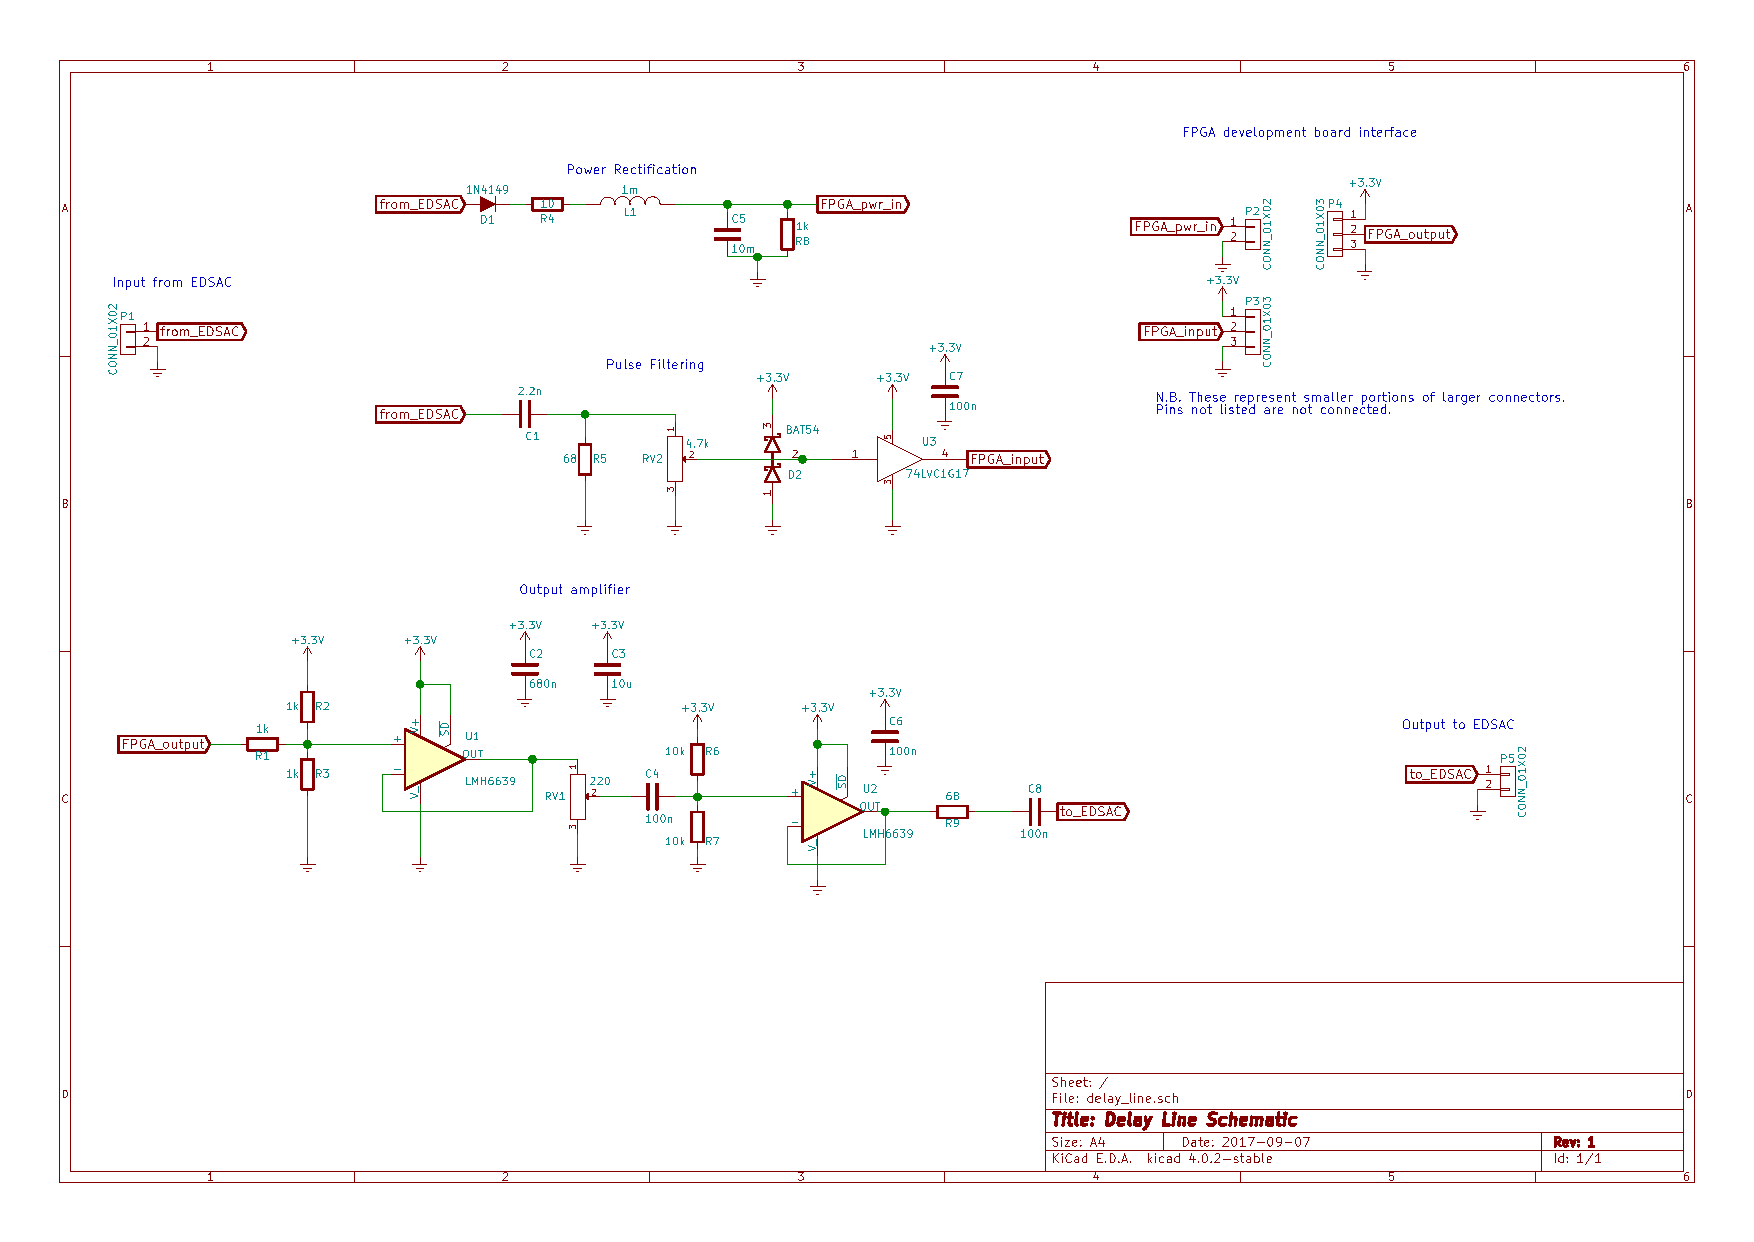
\includepdf[landscape]{figs/schematics/delay_line}
	\includepdf[landscape]{figs/schematics/test_harness}
%\end{landscape}


\chapter{\glsentryshort{hdl} verification results} \label{app:sim-wfms}
This appendix includes the the simulation waveforms resulting from verification.

The waveforms are included here since they are more clearly presented in landscape format, however they are discussed in Section \ref{sec:hdl-verif}.


\begin{landscape}

\begin{figure}[ht]
	\centering
	
	\begin{subfigure}[b]{\linewidth}
		\centering
		\includegraphics[width=\linewidth]{sim_results/delay_line/full_sim}
		\caption{Full Simulation}
		\label{fig:delay-sim-full}
	\end{subfigure}
	
	\begin{subfigure}[b]{\linewidth}
		\centering
		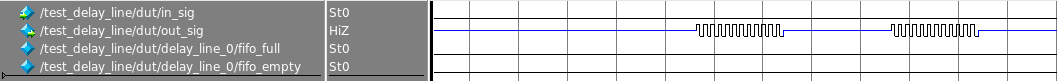
\includegraphics[width=\linewidth]{sim_results/delay_line/single_pulse}
		\caption{Simulated output of a single pulse}
		\label{fig:delay-sim-single}
	\end{subfigure}
	
	\caption{Delay Line Simulation Results}
	\label{fig:delay-sim}
\end{figure}

 \begin{figure}[ht]
	\centering
	\includegraphics[width=\linewidth]{sim_results/test_harness/full_sim}
	\caption{Full Simulation}
	\label{fig:harness-full}
\end{figure}

\end{landscape}

\end{appendices}

\end{document}